\documentclass{article}
    \usepackage{amssymb}
    \usepackage[utf8]{inputenc}
    \usepackage[russian]{babel}
    \usepackage[left=2cm,right=2cm,
        top=2cm,bottom=2cm,bindingoffset=0cm]{geometry}
    \usepackage{hyperref}
    \hypersetup{
        colorlinks=true,
        linkcolor=blue,
        filecolor=magenta,      
        urlcolor=cyan,
    }
  \usepackage{graphicx}
  \usepackage{booktabs}
  \usepackage{hyperref}
  \graphicspath{{pictures/}}
  \DeclareGraphicsExtensions{.pdf,.png,.jpg}
\usepackage{subcaption}
%\captionsetup{compatibility=false}

\begin{document}
\begin{center}{\hugeОтчет по дипломной работе за неделю\\}\end{center}
Дата: 22.4.2021\\
Научные руководители: Герасимов С.В., Мещеряков А.В.\\
Студент: Немешаева Алиса\\
Курс: 4\\

\renewcommand{\labelitemi}{$\blacksquare$}
\renewcommand\labelitemii{$\square$}

\begin{enumerate}
    \item Построены графики чистоты каталога (отношение найденных/ошибочных объектов) с 
        распределением по max\_pred.\\
    \item Исправлена старая версия презентации для выступления на Ломоносовских чтениях. 
        \href{https://github.com/rt2122/data-segmentation-2/blob/master/text/presentation_2021.4.22.pdf}{Ссылка}\\
\end{enumerate}

\begin{figure}[h]
    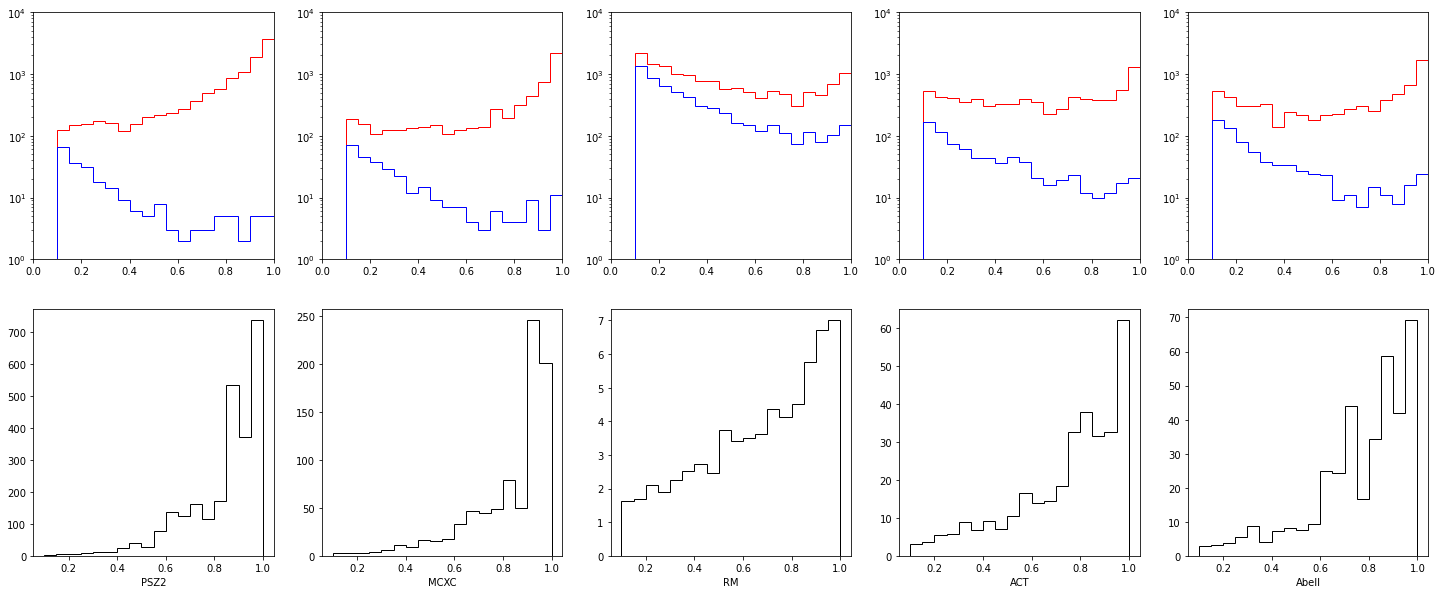
\includegraphics[width=\linewidth]{div}
\caption{Чистота каталога pz\_all\_found34 относительно параметра max\_pred.}
\label{Fig:div}
\end{figure}

Отчет согласован с научным руководителем.\\
Общее количество строк кода за эту неделю: 23\\
\href{https://github.com/rt2122/data-segmentation-2}{Репозиторий}\\ 
\end{document}
